\documentclass{article}
\usepackage{graphicx} % Required for inserting images

\title{phys-ga-2000-ps5}
\author{https://github.com/kdindial/phys-ga2000 }
\date{October 2024}

\begin{document}

\maketitle

\section{Problem 1}
See figure 1:
\begin{figure}[h!]
    \centering
    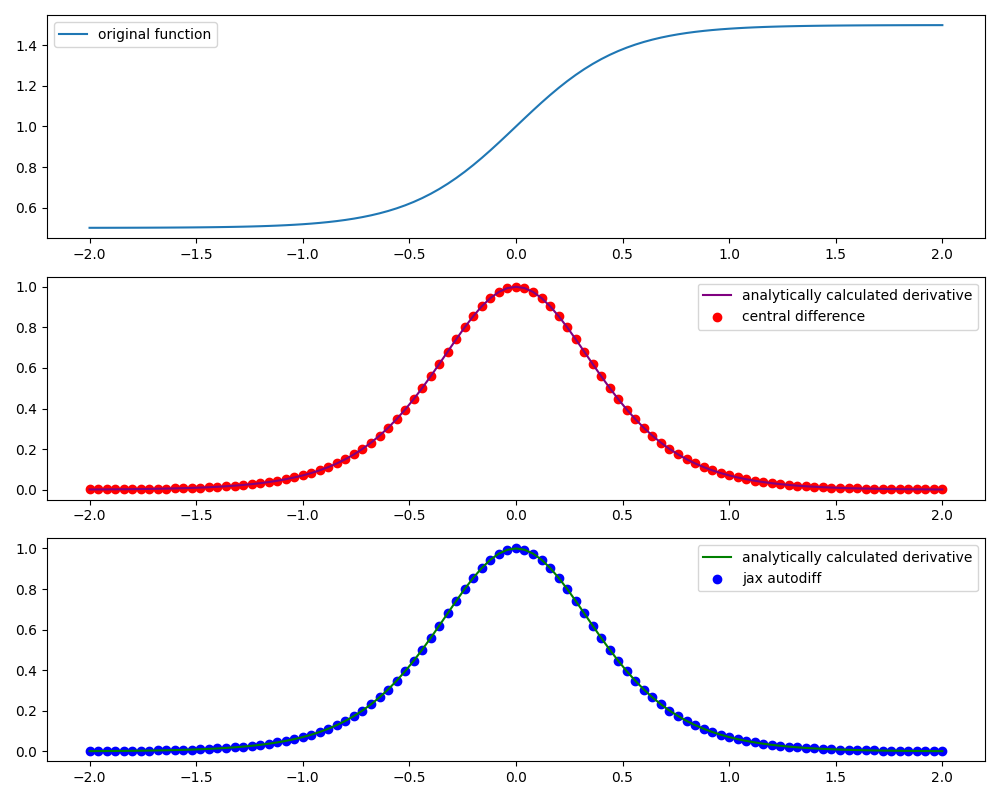
\includegraphics[width=0.5\linewidth]{ps5_figs/DifferentiationExample.png}
    \caption{Numerical Differentiation of $1+\frac{\tanh(2x)}{2}$}
    \label{fig:enter-label}
\end{figure}

\section{Problem 2}
\subsection{part a}

First we are asked to plot the integrand of the gamma frunction from x=0 to x=5 for 3 different a values. The gamma function is

\begin{equation}
    \Gamma(a)=\int_{0}^{\infty}x^{a-1}e^{-x}
\end{equation}

See Figure 2 for my plots

\subsection{part b}
Next we are asked to find the maximum of the integrand of equation 1, so I took its derivative and set it equal to 0:

\begin{equation}
    \frac{d}{dx}(x^{a-1}e^{-x})=(a-1)x^{a-2}e^{-x}-x^{a-1}e^{-x}=0
\end{equation}

factoring out the $e^{x}$ we get:
\begin{equation}
    (a-1)x^{a-2}-x^{a-1}=0
\end{equation}

which is equal to

\begin{equation}
    (a-1)x^{a-2}-x*x^{a-2}=0
    \end{equation}
Then factoring out the $x^{a-2}$
\begin{equation}
        a+1-x=0
\end{equation}
so $x=a-1$ at the critical point. To show that this point is a maximum, I would take the second derivative and plug in a-1 to see that it was negative at this point. But it is clear from Figure 2 that a-1 is a maximum.
\begin{figure}[t]
    \centering
    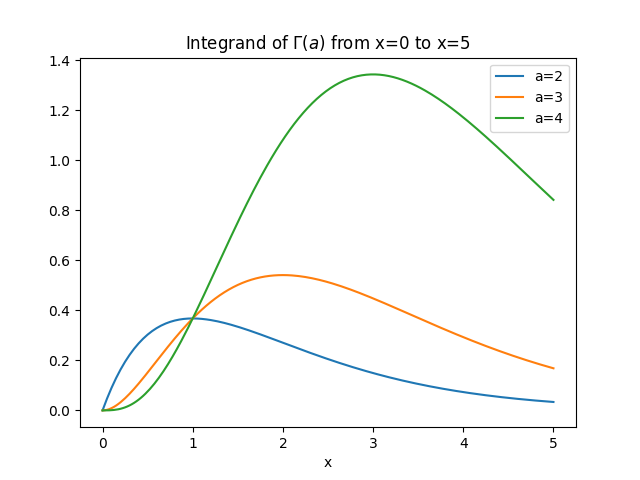
\includegraphics[width=0.5\linewidth]{ps5_figs/gamma_integrand.png}
    \caption{gamma function integrand}
    \label{fig:enter-label}
\end{figure}

\subsection{part c}
To numerically compute the integral. we are going to use the transformation:

\begin{equation}
    z=\frac{x}{x+c}
\end{equation}

We are asked to find which value of x gives z=1/2. Clearly it will be at x=c. We want the integrand maximum to be at z=1/2, so we should chose c=(a-1). 
\subsection{part d}
equation 1 could have potential problems when evaluating it numerically because for large x values you can have overflow in the power term and underflow and the exponential term. Instead we are asked to write the integrand as:

\begin{equation}
    e^{((a-1)\ln(x)-x}
\end{equation}

The new expression consolidates everything into a single exponential. This is more stable because for large values of x the computer instead evaluates (a-1)ln(x)-x, which avoids multiplying two numbers which could potentially cause an overflow or underflow.

\section{e and f}

computed gamma(3/2): 0.8862694302378595 \\
computed gamma(2): 1.0000050776228497 \\
computed gamma(3): 2.000002260422814 \\
computed gamma(5): 23.999997473153606 \\
computed gamma(9): 367895.76055080385 \\

\section{Problem 3}

\subsection{part a}
Figure 3 shows a plot of the raw data.


\begin{figure}[h]
    \centering
    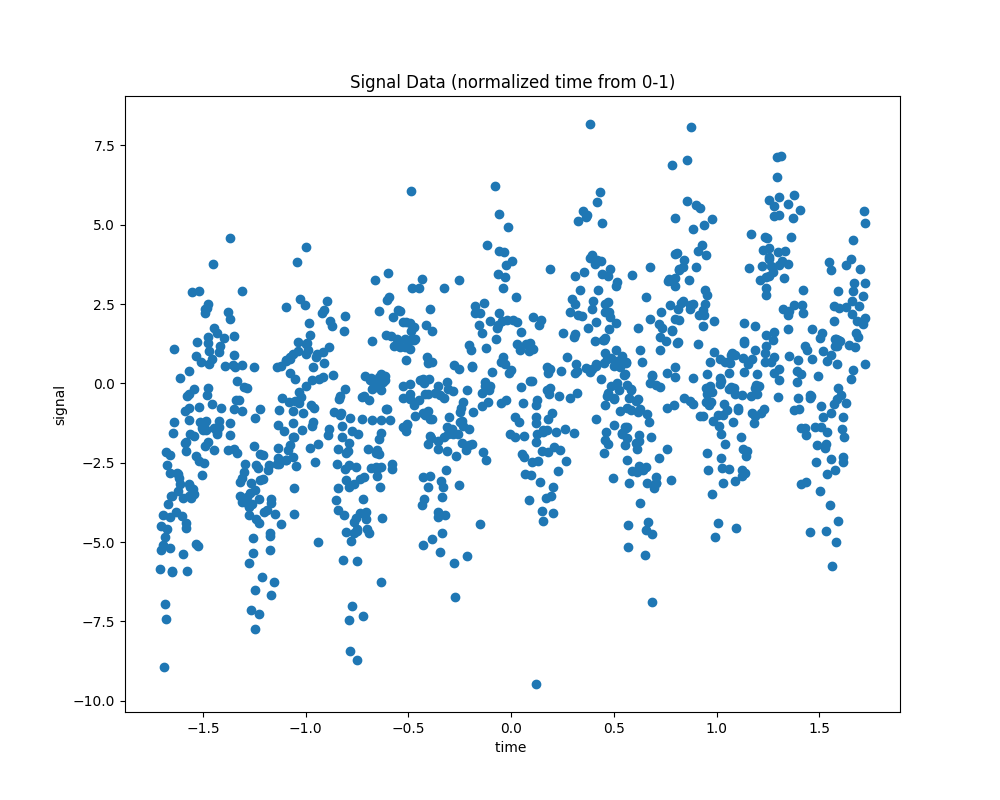
\includegraphics[width=.8\linewidth]{ps5_figs/3a.png}
    \caption{Raw Data (Normalized)}
    \label{fig:enter-label}
\end{figure}

\section{part b}
Figure 4 shows a 3rd order polynomial fit of the data
\begin{figure}[h]
    \centering
    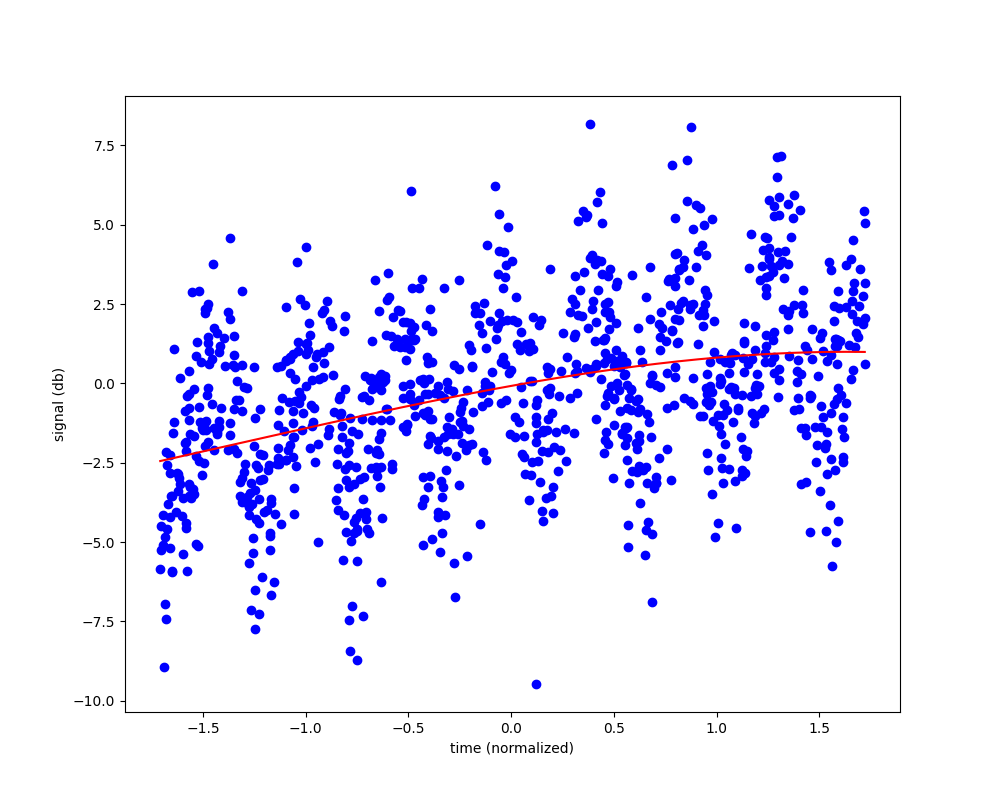
\includegraphics[width=.8\linewidth]{ps5_figs/3b.png}
    \caption{3rd Order Polynomial fit}
    \label{fig:enter-label}
\end{figure}

\subsection{part c}
\begin{figure}[h]
    \centering
    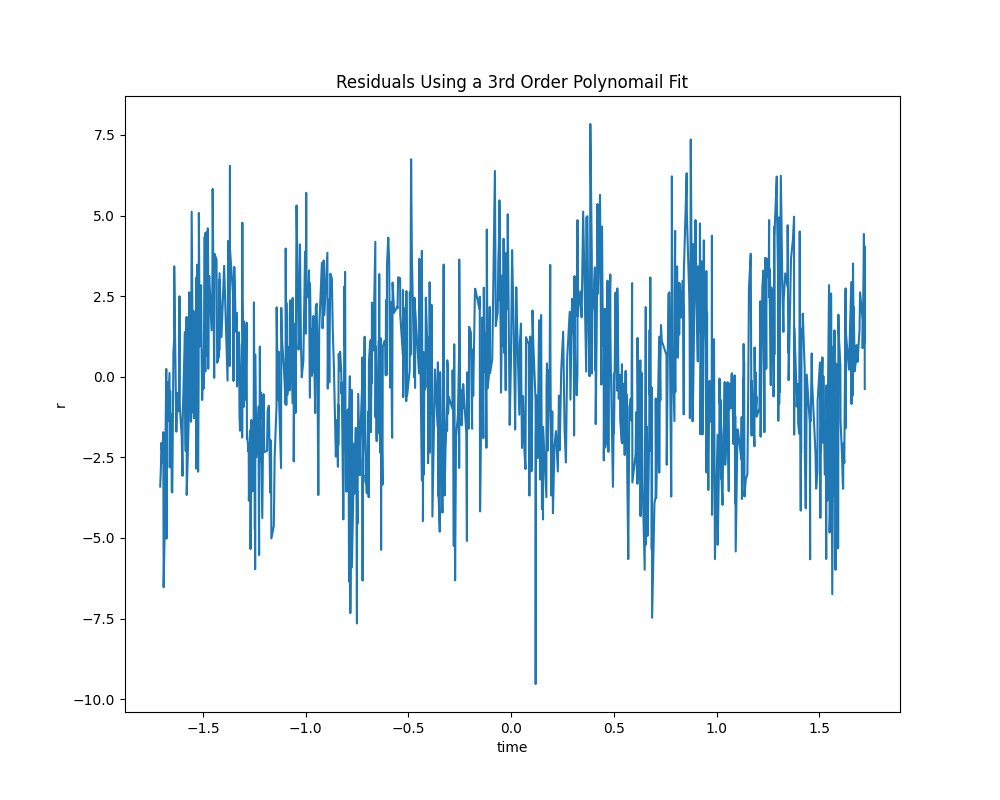
\includegraphics[width=0.8 \linewidth]{ps5_figs/3c.png}
    \caption{Residuals of 3d Order Polynomial fit}
    \label{fig:enter-label}
\end{figure}
The residuals have range of about $\pm8$ in the signal units, which is 4 times greater than the standard deviation. Clearly this is not a great fit. See Figure 5 for the residuals


\subsection{ part d}
For this section, I fit a 5th order polynomial, 10th order, 15th order and 20th order polynomial and plotted it in Figure 6.

\begin{figure}[t]
    \centering
    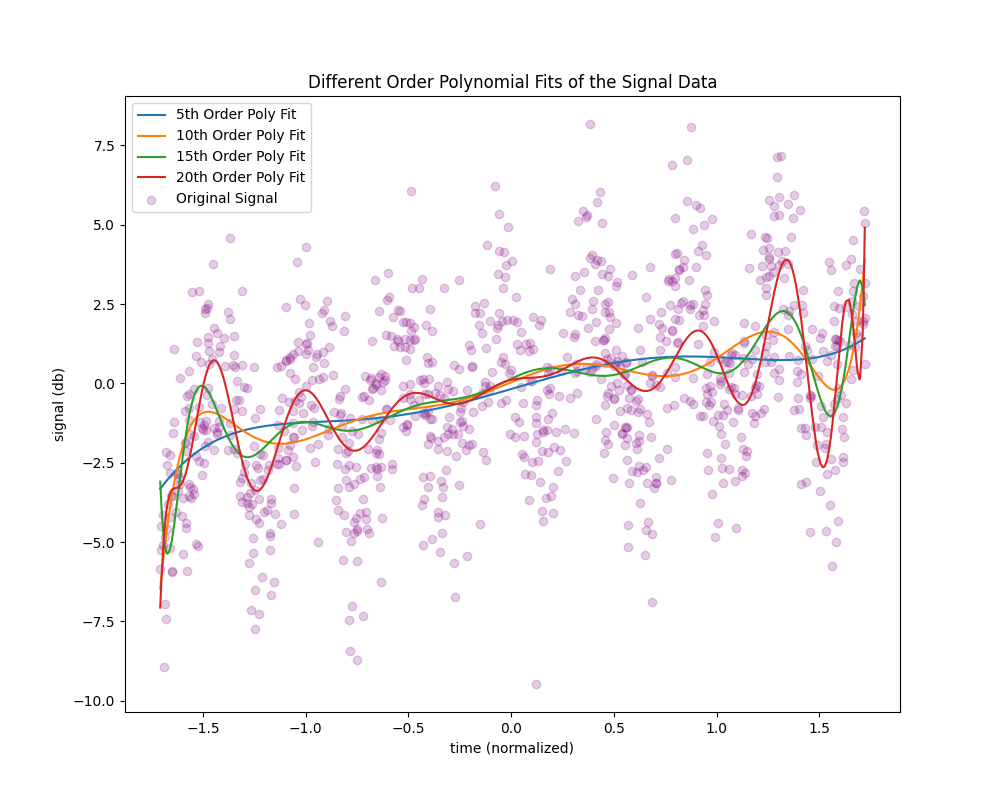
\includegraphics[width=0.8\linewidth]{ps5_figs/3d.png}
    \caption{Higher Order Polynomial Fits}
    \label{fig:enter-label}
\end{figure}

The condition number quickly becomes unreasonably large for higher order polynomials: \\
Condition number of the 5th order polynomial design matrix: 36.591702089964684 \\
Condition number of the 10th order polynomial design matrix: 5313.972718130102 \\
Condition number of the 15th order polynomial design matrix: 959548.2913040906 \\
Condition number of the 20th order polynomial design matrix: 189388894.17467415\\


Even though the higher order polynomials visually look like a slightly better fit, they are not viable fits because the condition number is way too high. 

\subsection{e}

Next, I fit to a harmonic series. I tried fitting with 10 modes, 200 modes, which can be seen in Figure 7. The 10 mode fit clearly captures the periodicity of the data. I tried fitting 200 modes just for fun, it is clearly "overfitting" the data but I thought it looked cool. When I printed out the coefficient matrix, the dominant terms were the 8th and 9th coefficients. The way I wrote my code, these correspond to sine and cosine terms with periods that are 1/8th the length of the data. Visually this makes sense, because you can count about 8 periods in the data. The condition number for the 10 mode fit was 1.62894179741679 and the condition number for the 200 mode fit was about 30.5, which is much more stable than the polynomial fit.

\begin{figure}[h]
    \centering
    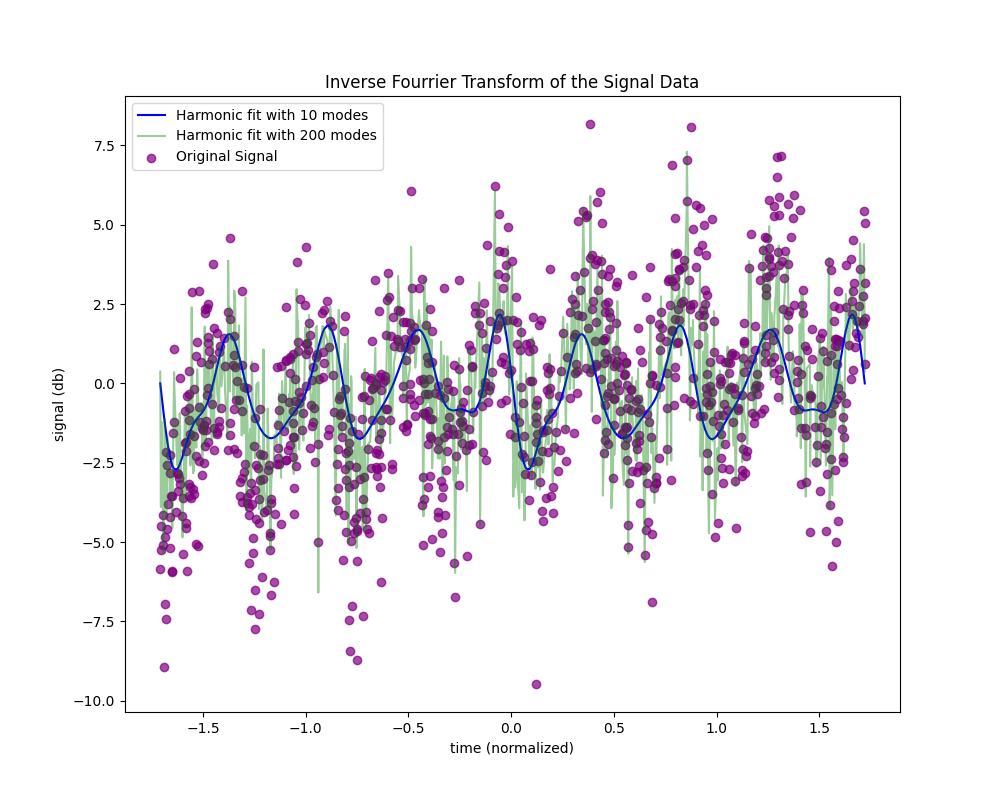
\includegraphics[width=0.8\linewidth]{ps5_figs/3e.png}
    \caption{Caption}
    \label{fig:enter-label}
\end{figure}

\end{document}
